\section{Preliminaries}
\subsection{Data Collection\label{sec:data}}
We collected crowdsourced segmentation data from Amazon Mechanical Turk where each HIT consisted of one segmentation task for a specific pre-labeled object in the image. There were a total of 46 objects in 9 images from the MSCOCO dataset~\cite{Lin2014}. For each object, we collected segmentation masks from a total of 40 workers. As shown in Fig.\ref{interface}, each task contains a semantic keyword and a pointer indicating the object to be segmented. These tasks represent a diverse set of task difficulty (different levels of clutteredness, occlusion, lighting) and levels of task ambiguity. 
\begin{figure}[ht!]
\centering
\fbox{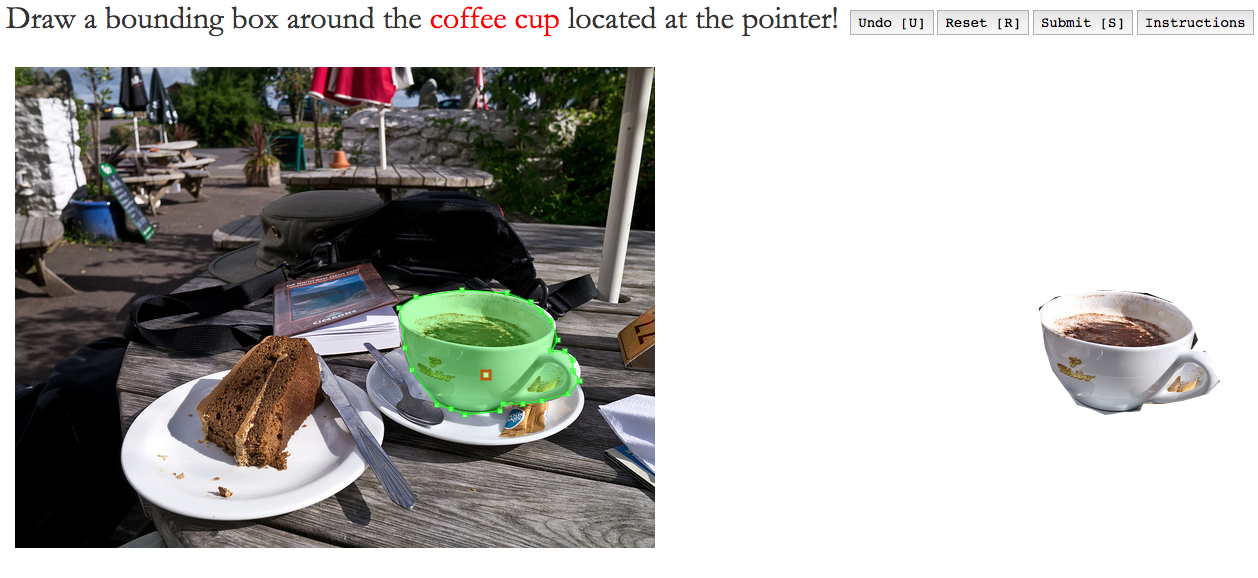
\includegraphics[width=0.9\linewidth]{plots/interface.png}}
\caption{An example interface for the segmentation webapp can be seen  \href{http://crowd-segment.herokuapp.com/segment/COCO_train2014_000000000127/10/}{here}.}
\label{interface}
\end{figure}
\subsection{Goal}
For any specified object in an image, there exists a {\em tight}\dor{why is specifying "tight" segmentation? Not sure purpose of this paragraph} segmentation  which exactly outlines the object; we call this the {\em ground-truth} segmentation for this object.  Workers are asked to provide segmentations for objects; they often do not provide the ground-truth segmentation,
and their segmentation is often noisy. Thus our goal is the following: given a raw image and multiple noisy worker segmentations for a specific object, estimate the ground truth segmentation for that object. \todo[inline]{Show one image + ground truth here} 
\subsection{Evaluation Metrics}
   \par Evaluation metrics used in our experiment measures how well the final segmentation (S) produced by these algorithms compare against ground truth (GT). The most common evaluation metric used in literature are area-based methods which take into account the intersection, $IA=area(S\cup GT)$, or union, $UA=area(S\cap GT)$, between the user and the ground truth segmentations. Specifically, we use
    $\text{Precision (P)} = \frac{IA(S)}{area(S)}$, 
    $\text{Recall (R)} = \frac{IA(S)}{area(GT)}$, and 
    $\text{Jaccard (J)} = \frac{UA(S)}{IA(S)}$
    metrics to evaluate our algorithms.